\documentclass[a4paper]{article}
\usepackage[utf8]{inputenc}  % si utf8
\usepackage{graphicx}
\usepackage{verbatim}

\pagestyle{plain}

\title{\textbf{Rapport de projet}\\- \Huge{Incidence} -}
\author{\emph{CHAMBONNET Kevin}\\\emph{GAUTHIER Silvère}\\\emph{MARTINEZ Thierry}\\\emph{MOKHRETAR Amin}}
\date{\today}

\newcommand{\alinea}{\hspace*{0.5cm}}

\begin{document}
  \maketitle
  \newpage
  \tableofcontents

  \newpage
  \part{Remerciements}

  \newpage
  \part{Cahier des charges}
  
    \section{Introduction}
    
    \section{Mecanismes de jeu}
    
    \section{Structure du jeu}
    
      \subsection{Moteur}
      
        \subsubsection{Moteur multi-agent}
        
        \subsubsection{Moteur de carte}
        
      \subsection{Scripts}
      
    \section{Elements graphiques}
    
    \section{Elements sonores}
    

  \newpage
  \part{Gestion du projet}
    \section{Gestion de l'équipe}
      \alinea Tous les membres se connaissant et étant supposés être capable de travailler en équipe, nous n'avons fait aucune élection de chef de projet.\\
      \alinea Nous avons opté pour travailler de manière collégiale, et ainsi garder une cohésion de groupe sans pour autant avoir de hiérarchie instaurée au sein du groupe, qui pourrait au contraire déservir la réalisation de nos objectifs.\\
      \alinea Chaque membre a donc autant de pouvoir que les autres, et peut donc participer activement au projet, autant lors de la conception que du développement. Toutes les décisions seront prises suivant la majorité lors de votes.\\\\
      \alinea Pour ce qui est des réunions de projets, nous avons convenu avec notre tuteur d'une réunion, allant d'environ trente minutes à une heure, toutes les une à deux semaines, afin de mettre au point l'avancement du projet. En parallèle, tous les membres de notre équipe se retrouvent une fois par semaine afin de discuter des points clés effectués ou à venir, donner lieu aux votes pour les prises de décisions, ou encore, lors de la phase de développement, travailler en collaboration afin d'optimiser notre travail.\\\\
      \alinea Au niveau du travail collaboratif, nous avons mis en place un dépôt sur github, contenant tant la documentation telle que ce rapport que les sources de notre jeu. Par ailleurs, nous mettrons sur ce dépôt uniquement les fichiers sources, les images et les sons, mais en aucun cas les fichiers temporaires ou les exécutables. Un fichier "makefile" sera disponible pour quiconque voudrait compiler le programme chez lui. Les seuls fichiers binaires disponibles seront les PDF de la documentation, pour un soucis de facilité d'accès.

    \section{Découpage en tâches}
      \alinea Afin de préparer le développement du jeu, il était nécessaire de séparer les fonctionnalités les unes des autres. Nous avons abouti à ce diagramme, qui résume notre choix de découpage :
      \begin{figure}
        \begin{center}
          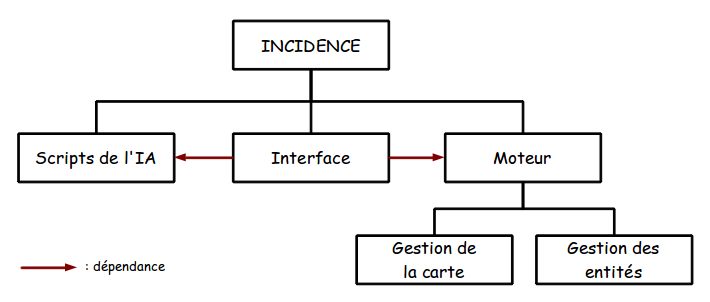
\includegraphics[scale=0.5]{img/DiagrammeDecoupageProjet.png}
        \end{center}
        \label{DiagDecoupage}
        \caption{Découpage du projet en sous-tâches}
      \end{figure}

    \section{Assignation}
      \alinea Le projet étant maintenant découpé en un certain nombre de modules, il ne restait plus qu'à assigner chaque tâche à un ou plusieurs membres de l'équipe. Nous nous sommes organisés comme ceci :
      \begin{itemize}
        \item \textbf{Scripts de l'IA :} MARTINEZ Thierry, MOKHRETAR Amin.
        \item \textbf{Moteur :}
        \begin{itemize}
          \item \textbf{Gestion de la carte :} GAUTHIER Silvère.
          \item \textbf{Gestion des entités :} CHAMBONNET Kevin.
        \end{itemize}
        \item \textbf{Interface :} Tous les membres.
      \end{itemize}
      \alinea Bien entendu, cette répartition n'est pas totalement fixée, elle concerne en réalité l'affectation de responsables de parties, qui seront en charge de celle-ci mais pourront évidemment faire appel aux autres membres pour trouver une solution à un problème par exemple.\\
      \alinea Le détail complet des tâches et assignations se situe dans la section Gestion du temps, page \pageref{GestionTps}.

    \section{Gestion du temps}
      \label{GestionTps}
      \alinea Afin de clarifier notre gestion du temps, un diagramme de Gantt est disponible dans la documentation de notre projet, et sera mis à jour en fonction de l'avancée du projet.\\
	  \newpage
      \begin{figure}
        \begin{center}
          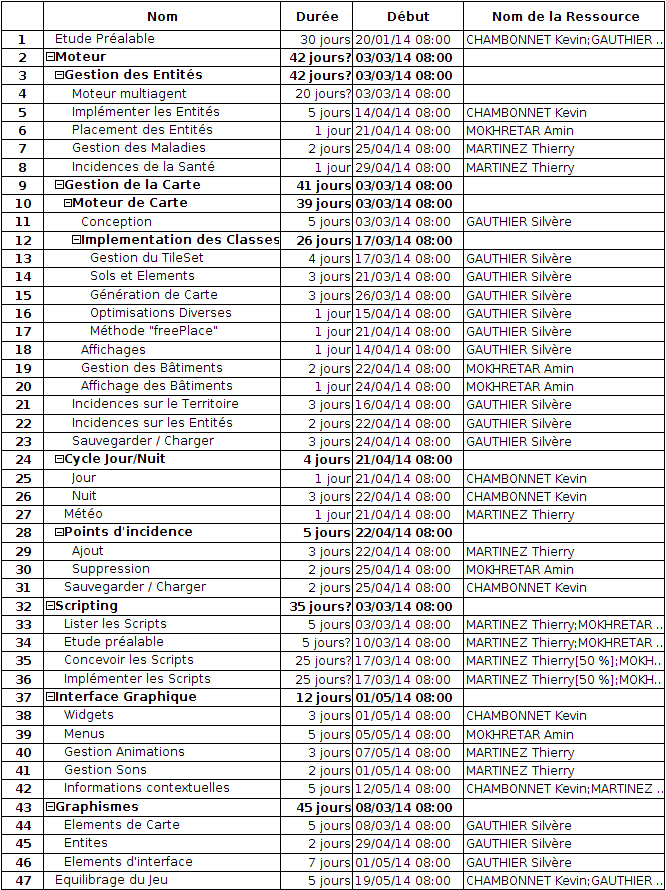
\includegraphics[scale=0.5]{img/gantt_1.png}
        \end{center}
        \label{DiagGantt}
        \caption{Diagramme de Gantt (page 1)}
      \end{figure}
      \newpage
      \begin{figure}
        \begin{center}
          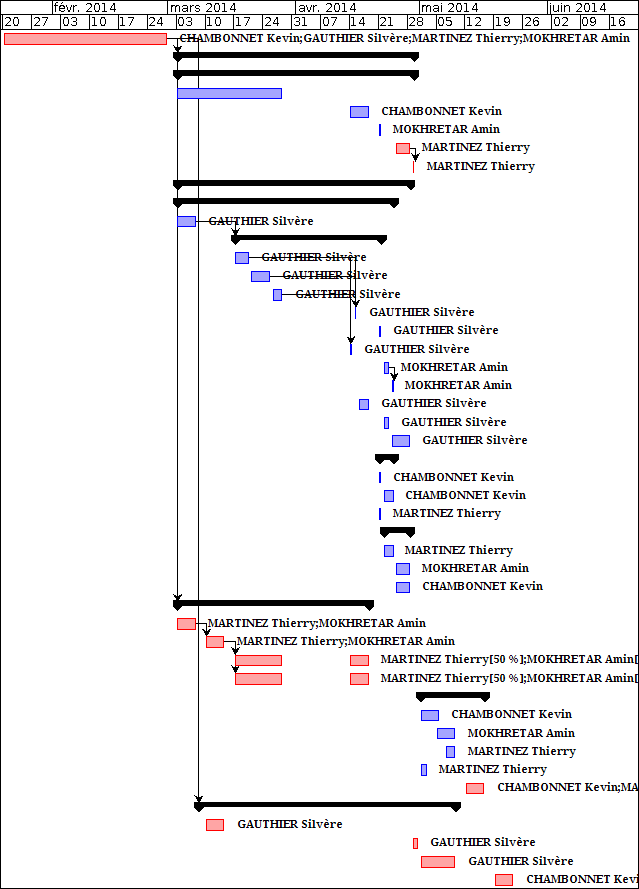
\includegraphics[scale=0.5]{img/gantt_2.png}
        \end{center}
        \caption{Diagramme de Gantt (page 2)}
      \end{figure}

    \section{Profil de risques}
      \begin{small}
        \begin{tabular}{| c | l |}
          \hline
          \textbf{Nature du risque} & \textbf{Degré du risque pour le projet}\\
          & 0 \hspace{0.5cm} 1 \hspace{0.5cm} 2 \hspace{0.5cm} 3 \hspace{0.5cm} 4 \hspace{0.5cm} 5\\
          \hline
          Taille du projet & \hspace{4.5cm} \circle*{5}\\
          \cline{1-1}
          Difficulté technique & \hspace{2.7cm} \circle*{5}\\
          \cline{1-1}
          Degré d'intégration & \hspace{2.25cm} \circle*{5}\\
          \cline{1-1}
          Configuration organisationnelle & \hspace{1.8cm} \circle*{5}\\
          \cline{1-1}
          Changement & \hspace{0.9cm} \circle*{5}\\
          \cline{1-1}
          Instabilité de l'équipe de projet & \hspace{0.9cm} \circle*{5}\\
          \hline
        \end{tabular}
      \end{small}

    \section{Choix technologiques}
      \subsection{Langages de programmation}
        \alinea Pour des besoins de performances, nous avons comparé différents langages. Pour réduire le temps de recherche et de comparaison, nous nous sommes appuyé sur des tests déjà effectués par d'autre.\\
        \alinea Voici des tests de performances concernant un large panel de langages, comparés ici dans quatre contextes différents :\\
        \begin{figure}
          \begin{center}
            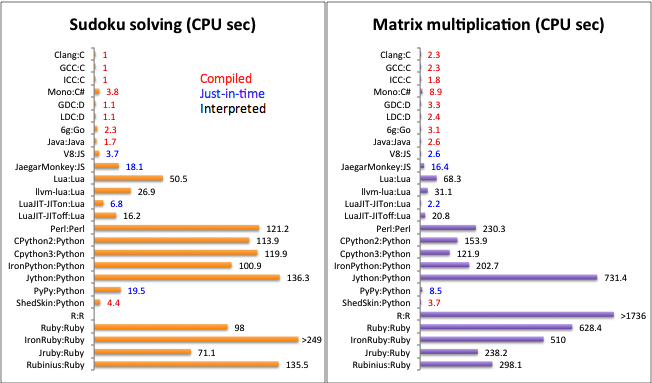
\includegraphics[scale=0.5]{img/AnalyseLangage1.png}
            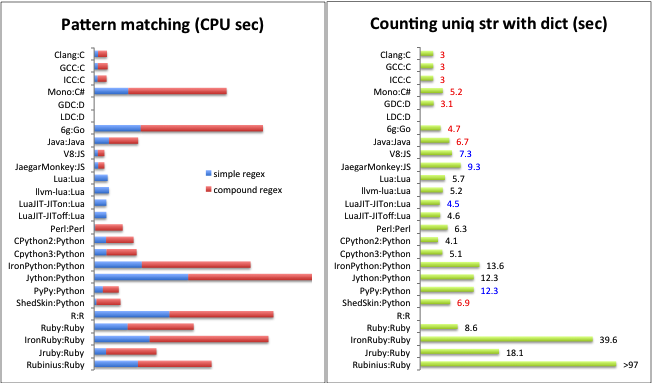
\includegraphics[scale=0.5]{img/AnalyseLangage2.png} 
          \end{center}
          \label{DiagAnalyse}
          \caption{Comparaisons de performances de divers langages dans des cas donnés}
        \end{figure}
        \alinea Nous pouvons observer que globalement, le langage le plus rapide est ici C++. L'utilisation de ce langage étant très fréquente dans les jeux vidéos, de part sa réputation d'un des langages les plus performants, et tous les membres de notre équipe sachant l'utiliser, nous avons fait le choix de programmer le moteur du jeu en C++.\\
        \alinea Afin d'optimiser encore la rapidité du moteur, nous avons cherché à associer son coeur écrit en C++ avec un langage de scripting qui permettra de mettre en place les différentes actions du jeu.\\ D'après les graphiques ci-dessus, nous avons opté pour le langage LUA, performant et facile d'utilisation (syntaxe proche du C++). En effet, même si Python est très prisé et offre beaucoup plus de possibilités que LUA, nous l'avons estimé bien trop lourd pour l'utilisation que nous allons en faire.\\
        \alinea Les deux langages C++ et LUA sont souvent associés dans les jeux vidéos, notre choix suit donc la tendance, ce qui nous offre une certaine assurance.

      \subsection{Bibliothèques}
        \alinea Pour la gestion graphique des tuiles composant la carte et des différentes entités, nous avons cherché une bibliothèque relativement simple d'utilisation mais surtout performante afin de garder la fluidité gagnée avec le choix des langages de programmation.\\
        \alinea Connaissant la bibliothèque OpenGL, qui est bas niveau et performante dans les affichages deux et trois dimensions, nous nous sommes tournés vers deux bibliothèques utilisant OpenGL : SDL et SFML.\\
        \alinea D'après plusieurs sites web et forums, les dernières versions (respectivement 2.0 et 2.1) de ces deux bibliothèques se valent en terme de performance.\\
        \alinea En confrontant nos préférences personnelles quant au choix de l'une ou l'autre, nous nous sommes finalement mis d'accord pour utiliser la bibliothèque graphique SFML 2.1, qui paraît plus simple d'utilisation que la SDL. De plus, elle permet une gestion aisée des fichiers audio, ce qui sera un plus pour la finalité de notre jeu.
      
    \section{Gestion des fichiers}
      \subsection{Format des Fichiers}
	    \alinea Le moteur de jeu étant écrit en C++, nous utiliserons des fichiers d'en-tête au format HPP et des fichiers de définition au format CPP. Pour les scripts d'IA des entités, le langage étant Lua, ceux-ci seront au format LUA.\\
        \alinea Toutes les images nécessaires au jeu seront au format PNG afin de pouvoir utiliser la transparence et garder la pleine qualité d'image (contrairement à JPEG qui perd de l'information à la compression).\\
        \alinea Les sons quant à eux seront au format WAV afin d'éviter toute gestion de la compression de fichier pour de petits fichiers qui n'en ont aucunement besoin.

        \subsubsection{Animation}
          \begin{verbatim}
            Chemin/vers/image.png size_x_sprite size_y_sprite play?(1/0) loop?(1/0)
            +Frame position_x position_y temps_affichage
            +Frame position_x position_y temps_affichage
            +Frame position_x position_y temps_affichage
          \end{verbatim}
      
        \subsubsection{Tileset}
	      \alinea Le tileset sera une unique image au format PNG représentant l'ensemble des tuiles possibles. Chaque type de sol constituera une ligne du tileset, avec toutes les variantes dépendant des rebords entre tuiles (ce fichier sera présenté plus en détails dans la section \ref{TilesetDev}, page \pageref{TilesetDev}).

        \subsubsection{Carte}
	      \alinea Les différentes cartes sauvegardées seront enregistrées dans des fichiers IMS (Incidence Map Save), dans lesquels seront stockés le tileset utilisé et la conformation de la carte (dimensions, sols et éléments).
      
        \subsubsection{Sauvegarde}
		  \alinea Un fichier sera créé pour la savegarde du jeu et un autre pour la sauvegarde de la carte, cela permettant dans le futur de créer des cartes réutilisables, comme par exemple dans un éditeur de carte.\\
		  \\
		  \alinea %TODO
		  \\
		  \alinea Le fichier de carte contiendra uniquement le lien vers le tileset ainsi que les types de sols et éléments présents sur la carte. Le fichier sera donc de la taille : 2 * nombre\_de\_cases * sizeof(int) + sizeof(chemin\_du\_tileset).\\
      
      \subsection{Commentaires}
        \alinea Si une méthode ou fonction, voir même un bloc, dépasse une certaine taille (environ 10 lignes) ou devient trop compliquée, un commentaire sera ajouté avant celle-ci expliquant brièvement son processus :
        \begin{verbatim}
          /** Description :
          *** Entrée : ...
          *** Sortie : ...
          **/
        \end{verbatim}
        \begin{small}
          \begin{tabular}{| c | c |}
            \hline
            \textbf{Marqueur spécifique} & \textbf{Signification}\\
            \hline
            TODO & A mettre à la place du code d'une fonctionnalité à implémenter\\
            \hline
            RECODE & A mettre au dessus du bloc d'une fonctionnalité à refaire\\
            \hline
            FIXME & A mettre au dessus du bloc d'une fonctionnalité contenant un bug\\
            \hline
          \end{tabular}
        \end{small}

      \subsection{Convention de Nommage}
        \begin{small}
          \begin{tabular}{| c | c |}
            \hline
            \textbf{Type de variable} & \textbf{Format du nom}\\
            \hline
            Classe & Majuscule suivit de minuscules\\
            \hline
            Méthode & Minuscules (pour les mots composés,\\
            et & chaque mots suivant est\\
            Fonction & une majuscule suivit de minuscules)\\
            \hline
            Attribut de classe & m\_\\
            \hline
            Variable globale & g\_\\
            \hline
          \end{tabular}
        \end{small}

      \subsection{Gestion du code source}
        \alinea Afin de faciliter le travail collaboratif, nous utilisons un dépôt utilisant le gestionnaire de version GIT, hébergé sur le site https://github.com/. Sur ce dépôt seront présents tous les fichiers sources nécessaires au développement du jeu ainsi que les documentations au format Latex et PDF (même si aucun fichier binaire ne devrait être présent, il est plus pratique de récupérer directement un tel fichier que de le compiler soit-même). De plus, y seront stockées toutes les données utilisées par le jeu telles que les images et les sons. Seuls les fichiers temporaires, exécutables et fichiers de sauvegarde ne seront pas stockés.
		

  \newpage
  \part{Développement}
  
    \section{Moteur de jeu}
    
      \subsection{Gestion des états}
      
      \subsection{Gestion de l'interface utilisateur}
      
      \subsection{Gestion des ressources et animations}
      
	\section{Moteur de carte}
      \subsection{Les Tuiles}
        \alinea Les différents types de tuile seront tous recensés dans le tileset, qui se chargera de fournir les textures et attributs associés à ceux-ci. La carte n'utilisera que des pointeurs vers ces instances constantes de tuile, ce  qui évitera le stockage inutile d'instances identiques.
        
        \subsubsection{Les Sols}
          \alinea Chaque sol aura différents attributs définis dans le fichier de configuration du tileset (cf section \ref{TilesetDev}, page \pageref{TilesetDev}). Comme définis dans le cachier des charges, certains sols seront incompatibles avec d'autres.\\
          \\
	  	  \begin{small}
			\begin{tabular}{| c | l |}
			  \hline
			  \textbf{Attribut} & \textbf{Description}\\
			  \hline
			  Type & Entier définissant un identificateur du type de sol.\\
			  \hline
			  Coût & Entier définissant le coût en PI de la pose du sol.\\
			  \hline
			  Nom & Chaîne de caractères utilisées lors des affichages dans l'interface.\\
			  \hline
			  Comportement & Enumération de trois comportements :\\
			  & DEFAULT : comportement par défaut (tous les type de Terre).\\
			  & FLUID : les sols forment des zones (étendues d'eau).\\
			  & CLIFF : les sols sont fixes et forment des zones (falaises).\\
			  \hline
			  Franchissable & Booléen indiquant si le sol est franchissable ou non par les unités.\\
			  \hline
			  Rebords & Tableaux d'entiers indiquant tous les types de sol compatibles\\
			  & avec les bordures de l'image (cf  section \ref{TilesetDev}, page \pageref{TilesetDev}).\\
			  \hline
			\end{tabular}
		  \end{small}
          
        \subsubsection{Les Eléments}
          \alinea Chaque sol aura différents attributs définis dans le fichier de configuration du tileset (cf section \ref{TilesetDev}, page \pageref{TilesetDev}).\\
          \\
	  	  \begin{small}
			\begin{tabular}{| c | l |}
			  \hline
			  \textbf{Attribut} & \textbf{Description}\\
			  \hline
			  Type & Entier définissant un identificateur du type d'élément.\\
			  \hline
			  Type de sol & Entier définissant un identificateur du type de sol sur lequel se place l'élément.\\
			  \hline
			  Coût & Entier définissant le coût en PI de la pose de l'élément.\\
			  \hline
			  Nom & Chaîne de caractères utilisées lors des affichages dans l'interface.\\
			  \hline
			  Comportement & Enumération de deux comportements :\\
			  & DEFAULT : comportement par défaut.\\
			  & FOREST : les éléments forment des zones (arbres).\\
			  \hline
			  Franchissable & Booléen indiquant si le sol est franchissable ou non par les unités.\\
			  \hline
			  Temps de récolte & Valeur de temps durant laquelle le citoyen doit agir afin de récolter les ressources.\\
			  \hline
			  Ressources & Ressources (et leur quantité) associées à l'élément.\\
			  \hline
			\end{tabular}
		  \end{small}
          
          
      \subsection{Le Tileset}
		\label{TilesetDev}
		\alinea Un unique fichier image au format PNG contiendra l'ensemble des tuiles utilisées dans le jeu pour les sols ou éléments. Cette image sera utilisée comme texture et certaines parties seront extraites par le programme au gré des besoins.
		\alinea Dans le but de permettre à l'utilisateur d'aisément créer des mods de jeu ou changer de tileset, nous avons créé un fichier au format INI détaillant toutes les particularités du tileset.\\
		\alinea Voici le tileset que nous utiliserons :\\
        \begin{figure}
          \begin{center}
            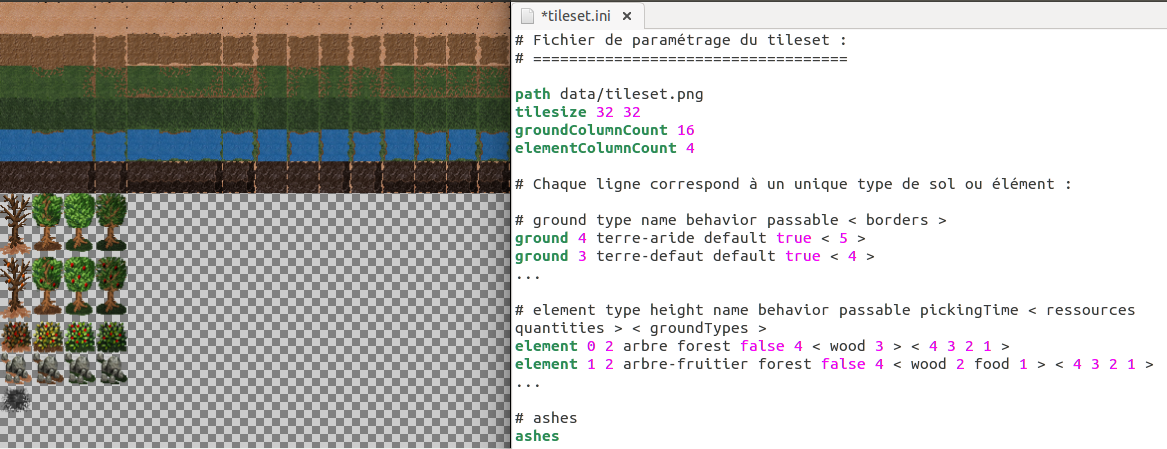
\includegraphics[scale=0.35]{img/TilesetPngIni.png}
          \end{center}
          \label{TilesetPngIni}
          \caption{Texture et configuration du tileset}
        \end{figure}
        \\
        \textbf{Fichier de configuration :}\\
        \alinea Chaque ligne commençant par "\#" ne sera pas lue, ce sont les commentaires. Les mots en vert sont les mots clés utilisés pour la lecture qui se fait ligne par ligne :\\
        - path : indique le chemin du fichier de texture du tileset\\
        - tilesize : est suivi des dimensions (en pixel, largeur puis hauteur) d'une tuile\\
        - groundColumnCount : nombre de colonnes pour chaque sol dans le fichier de texture (toutes les associations de rebords)\\
        - elementColumnCount : nombre de colonnes pour chaque élément dans le fichier de texture (tous les types de sols)\\
        - ground : définit un sol et tous ses attributs\\
        - element : définit un élément et tous ses attributs (height est la hauteur en nombre de cases dans la texture)\\
        - ashes : fourni une texture pour les cendres (lorsque des éléments brûlent) (cf GDD)\\
        \\
        Remarque : chaque ligne commençant par ground, element ou ashes incrémente un compteur afin de connaître la position de la zone de texture correspondante. L'ordre est donc important (définition des lignes de haut en bas).

      \subsection{Météo}
      
      \subsection{Incidences}
        \subsubsection{Dilatation}
          \alinea Les incidences basées sur la dilatation des zones prennent en compte les types de sols ou éléments afin d'élargir les étendues voulues en propageant les sols si besoin afin de garder les contraintes définies dans le GDD.\\
          \alinea Voici quelques présentations des résultats de ces dilatations :\\
        
        \subsubsection{Erosion}
          \alinea Les incidences basées sur l'érosion des zones prennent en compte les types de sols ou éléments alentours afin de choisir les types en propageant les sols si besoin afin de garder les contraintes définies dans le GDD.\\
          \alinea Voici quelques présentations des résultats de ces érosions :\\
        
        \subsubsection{Aléatoire}
          \alinea Les dernières incidences concernant le territoire sont basées sur un choix aléatoire de cases. Il s'agit ici d'appartition ou disparition de certaines ressources.\\
          \alinea Voici quelques résultats de ces incidences particulières :\\

	\section{Moteur multi-agent}
	
		\subsection{Gestion des entités}
		
			\subsubsection{Santé}
			
			\subsubsection{Incidences}
			
		\subsection{Gestion des scripts}
		
		\subsection{Liste des scripts}
		
	\section{Architecture}
	
		\subsection{Machine à états}
			pour chaque etat :
			interface + graphiques + sons + action possibles
	

  \newpage
  \part{Post-Mortem}
  
	\section{Réalisations non abouties}
	
	\section{Améliorations réalisables}
	

  \newpage
  \part{Annexes}
	\begin{figure}
	  \begin{center}
		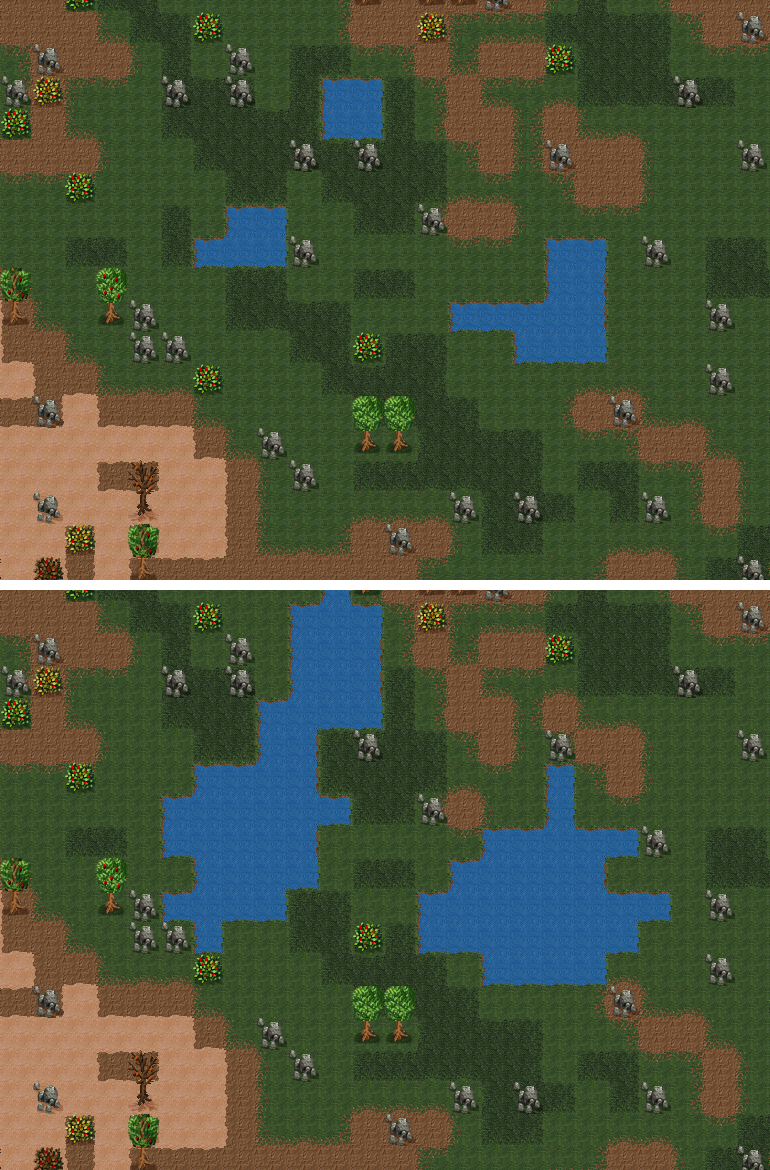
\includegraphics[scale=0.45]{img/DilateFluid.png}
	  \end{center}
	  \caption{Dilatation des étendues de fluides}
	\end{figure}
	\begin{figure}
	  \begin{center}
		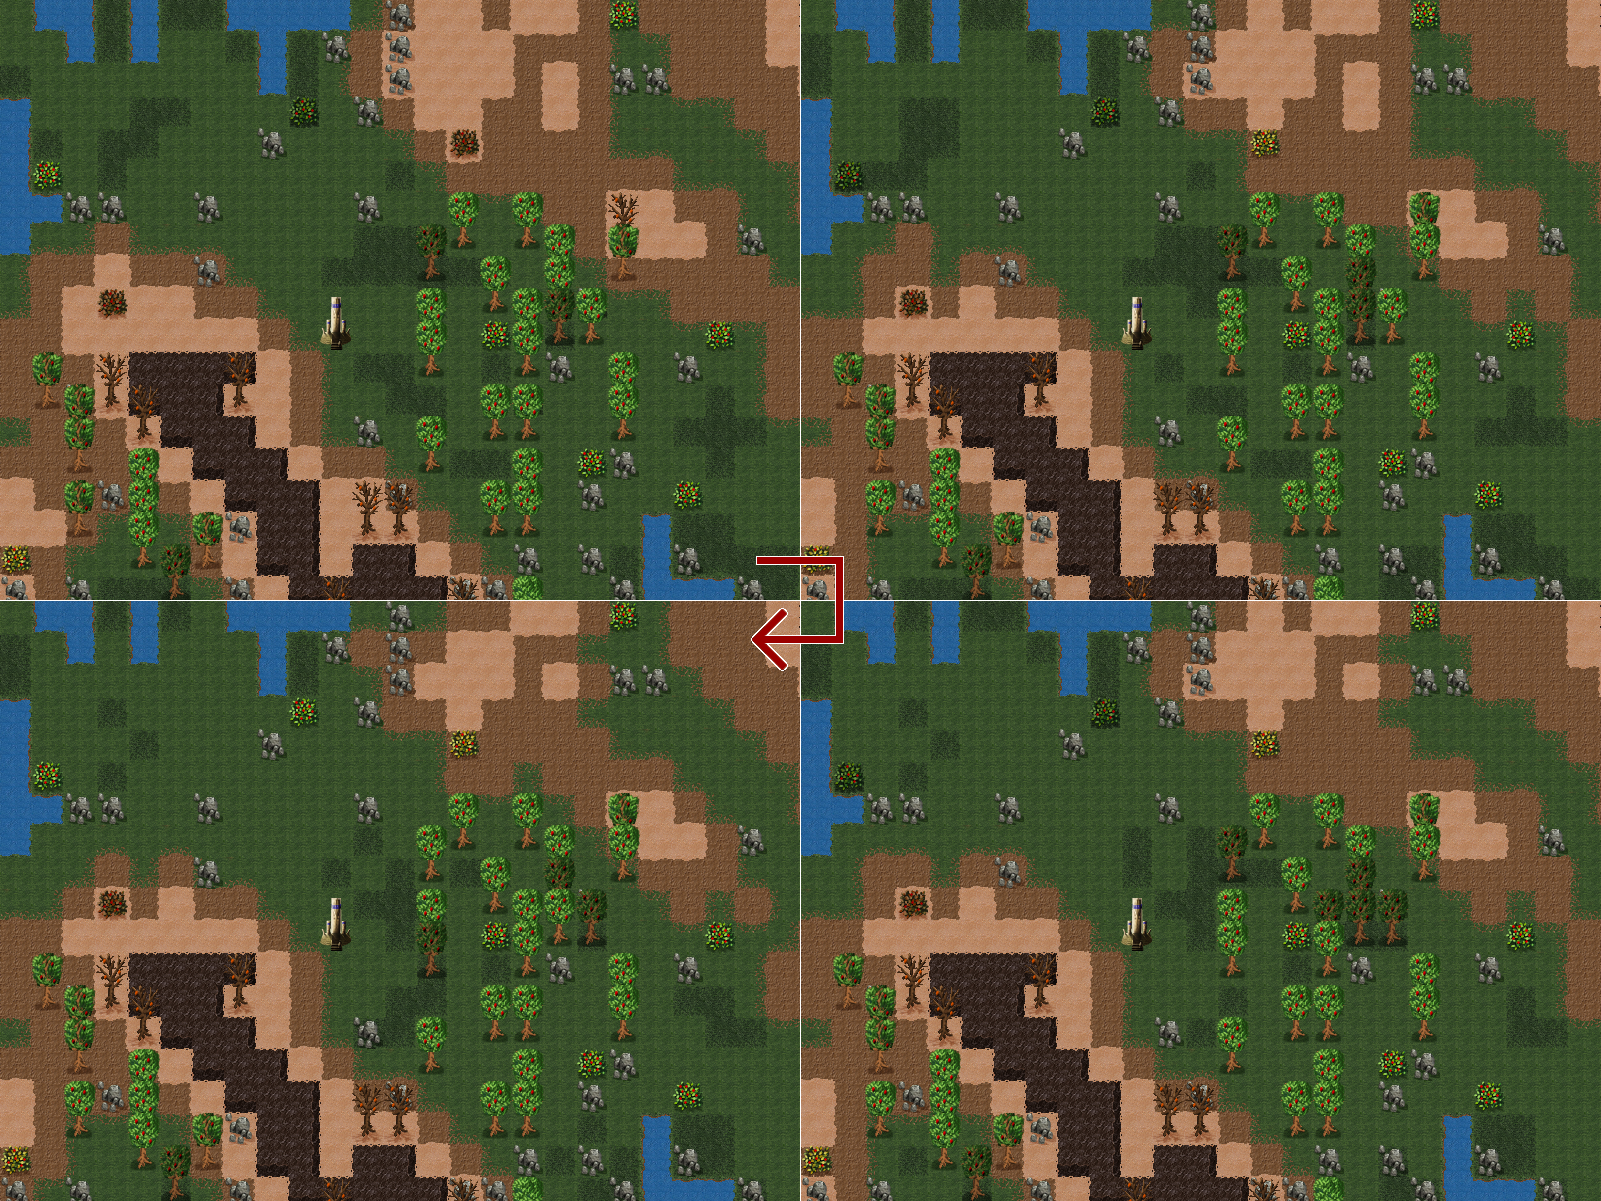
\includegraphics[scale=0.45]{img/DilateNearFluid.png}
	  \end{center}
	  \caption{Dilatation des zones humides}
	\end{figure}
	\begin{figure}
	  \begin{center}
		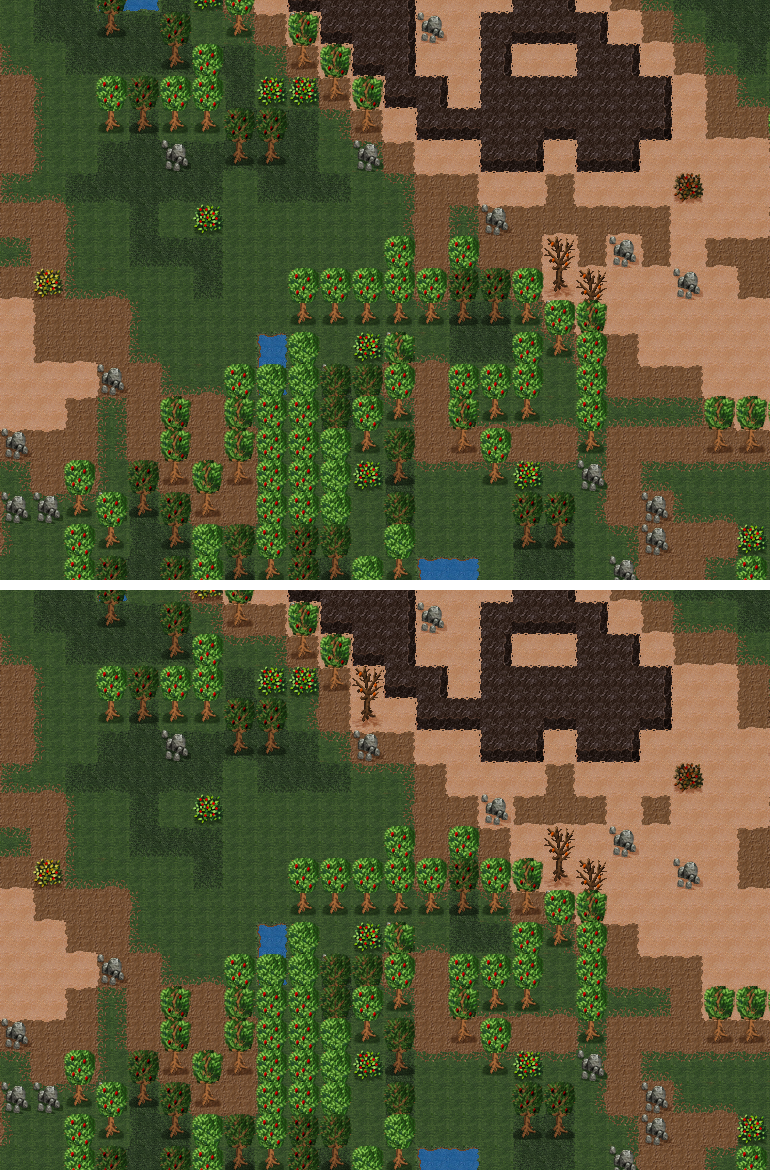
\includegraphics[scale=0.45]{img/DilateNearCliff.png}
	  \end{center}
	  \caption{Dilatation des zones sèches}
	\end{figure}
	\begin{figure}
	  \begin{center}
		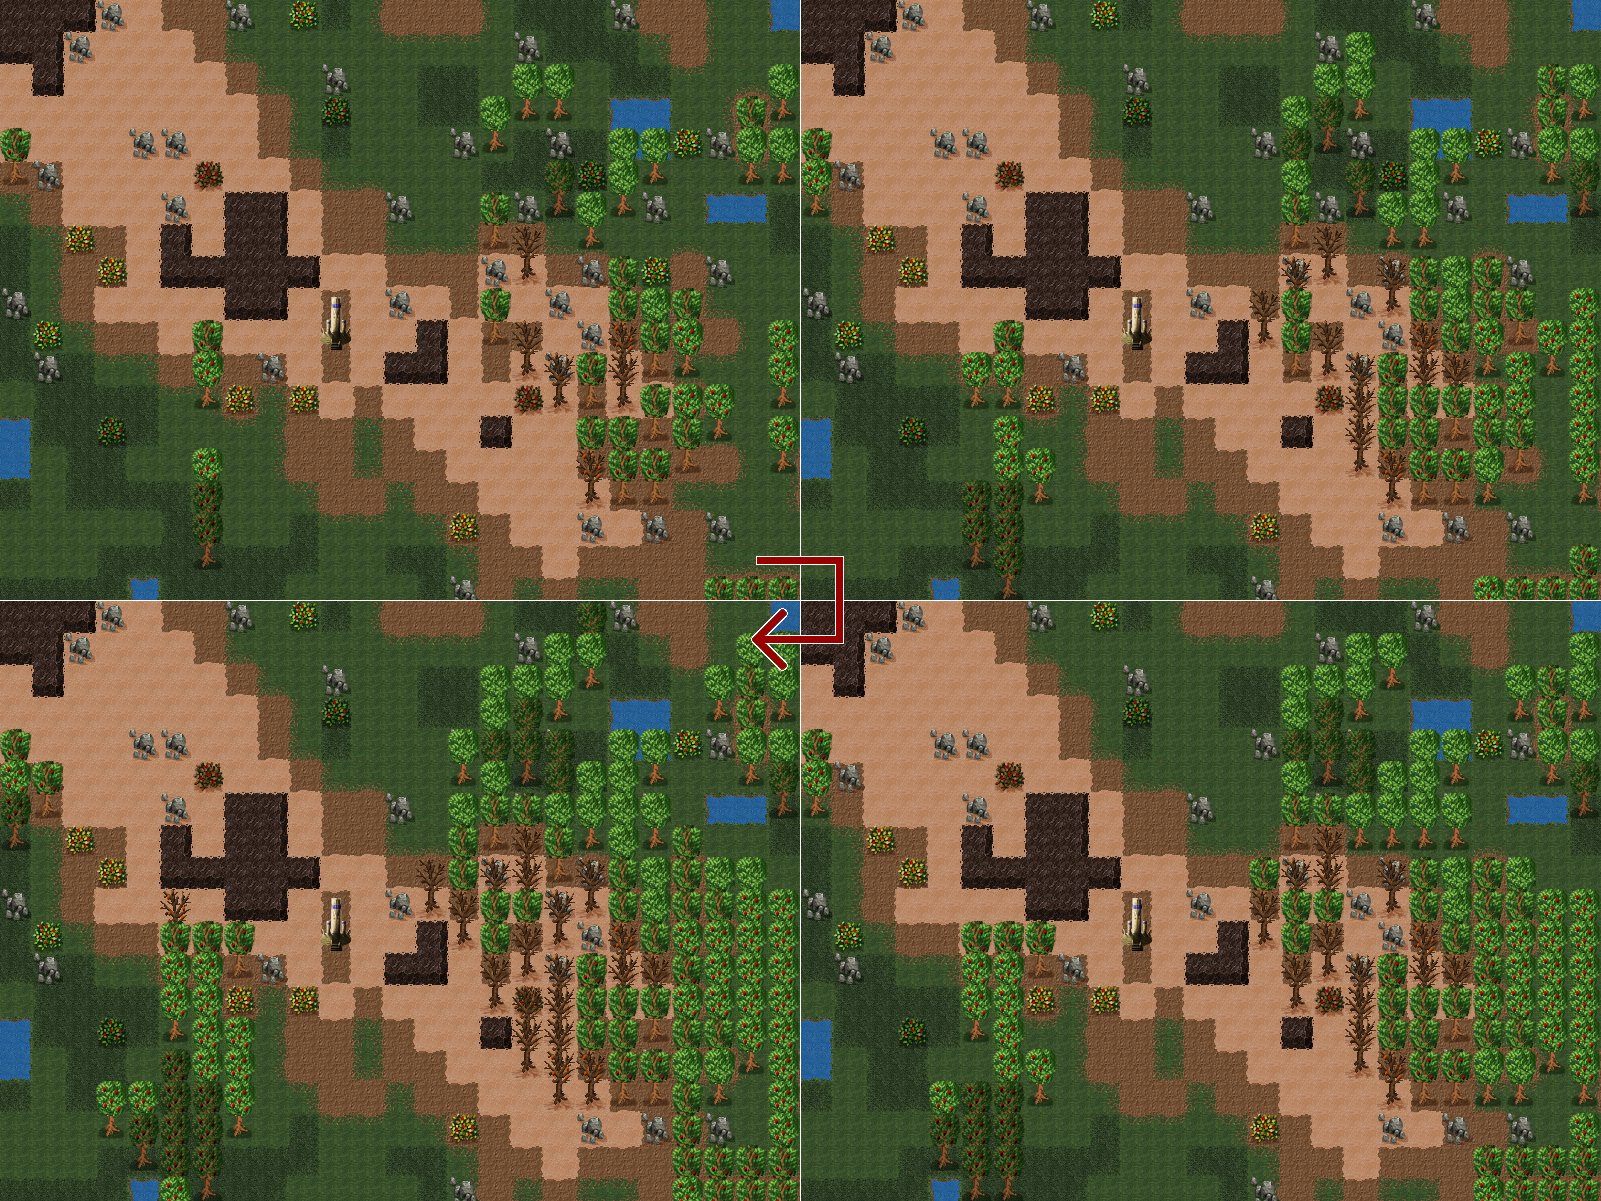
\includegraphics[scale=0.45]{img/DilateForest.png}
	  \end{center}
	  \caption{Dilatation des forêts}
	\end{figure}
	\begin{figure}
	  \begin{center}
		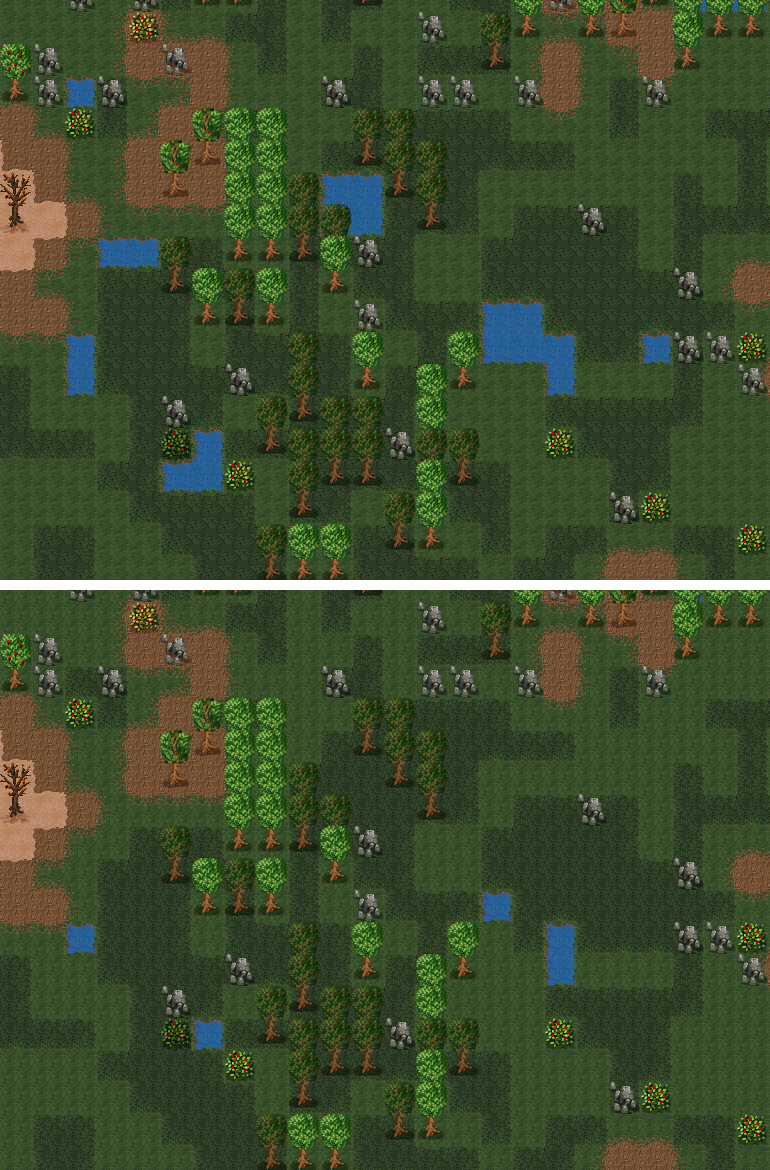
\includegraphics[scale=0.45]{img/ErodeFluid.png}
	  \end{center}
	  \caption{Erosion des étendues de fluides}
	\end{figure}
	\begin{figure}
	  \begin{center}
		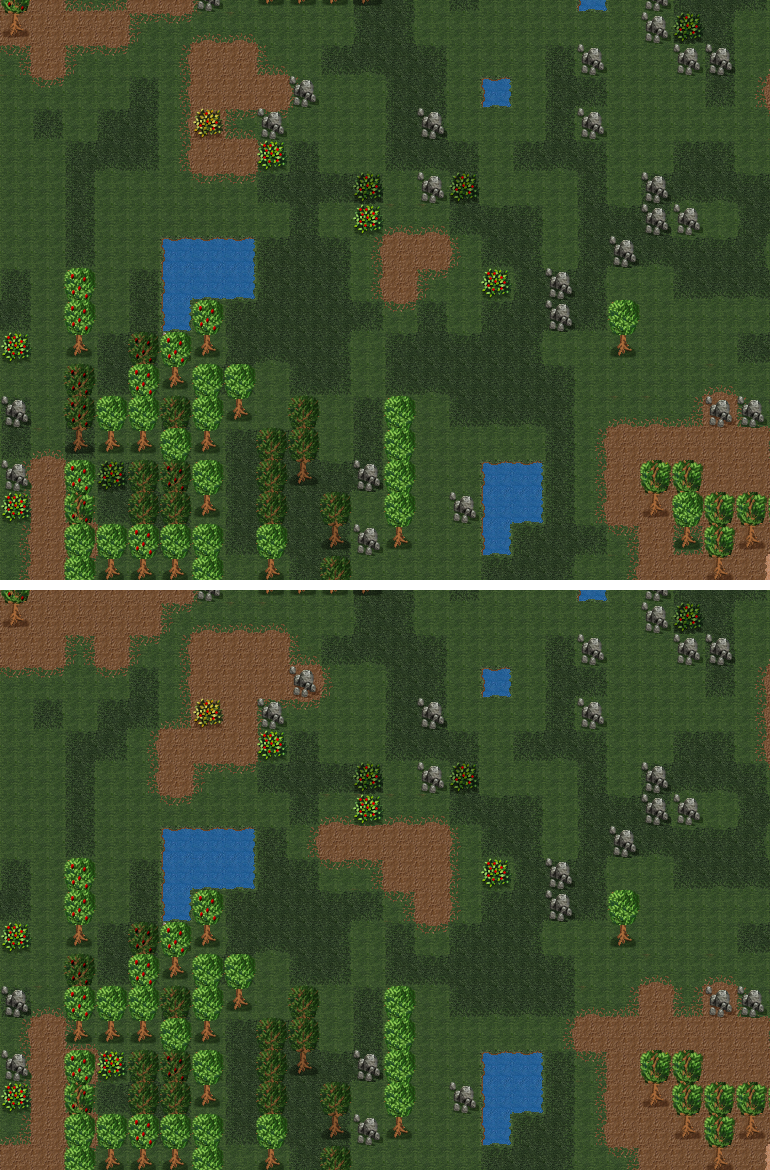
\includegraphics[scale=0.45]{img/ErodeNearFluid.png}
	  \end{center}
	  \caption{Erosion des zones humides}
	\end{figure}
	\begin{figure}
	  \begin{center}
		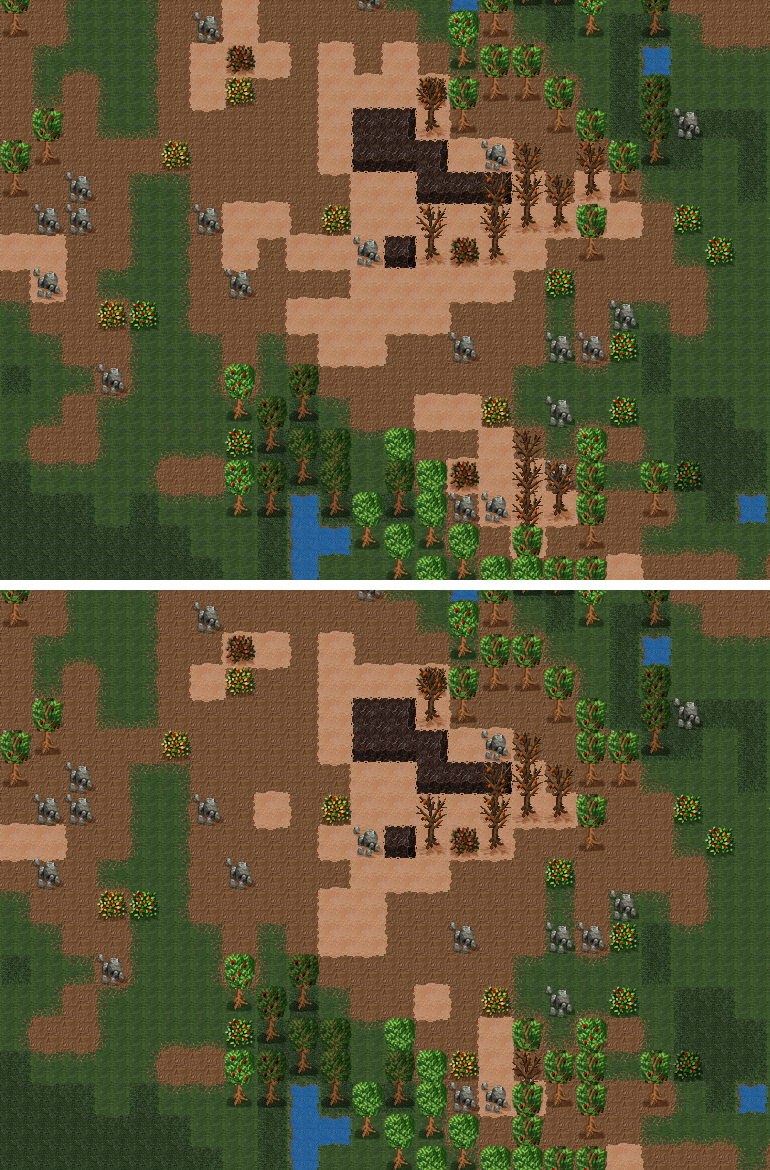
\includegraphics[scale=0.45]{img/ErodeNearCliff.png}
	  \end{center}
	  \caption{Erosion des zones sèches}
	\end{figure}
	\begin{figure}
	  \begin{center}
		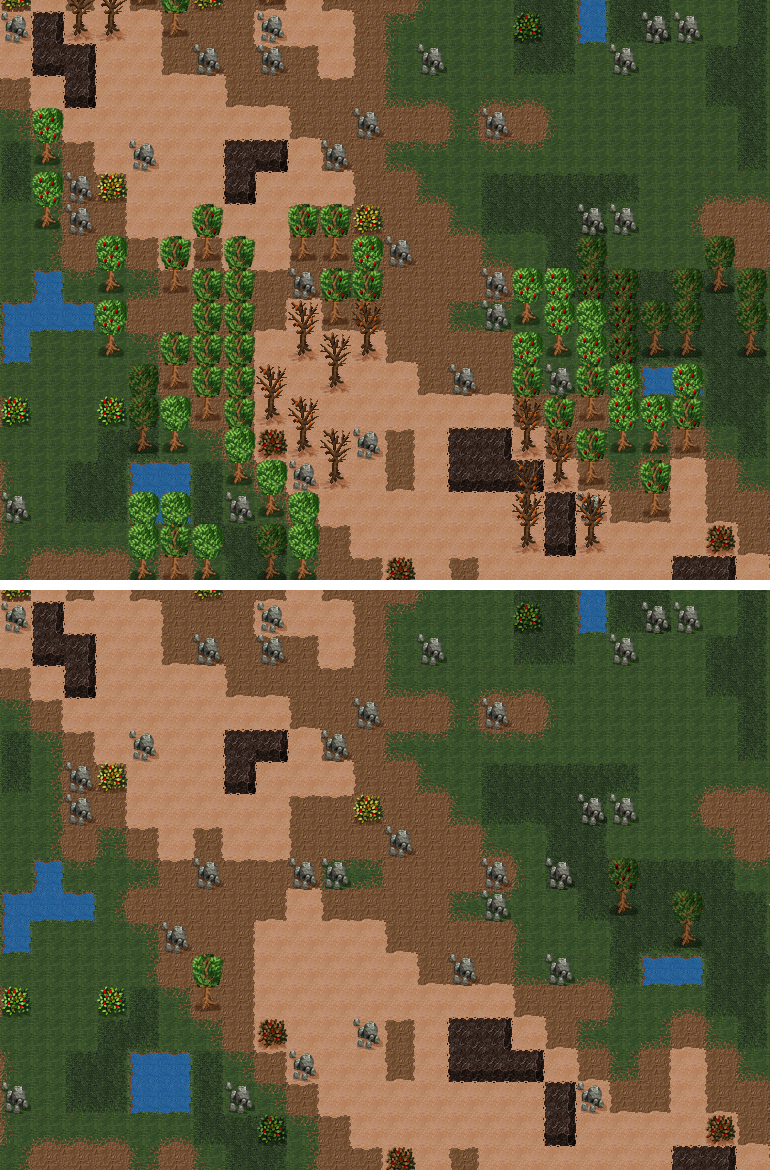
\includegraphics[scale=0.45]{img/ErodeForest.png}
	  \end{center}
	  \caption{Erosion des forêts}
	\end{figure}
	\begin{figure}
	  \begin{center}
		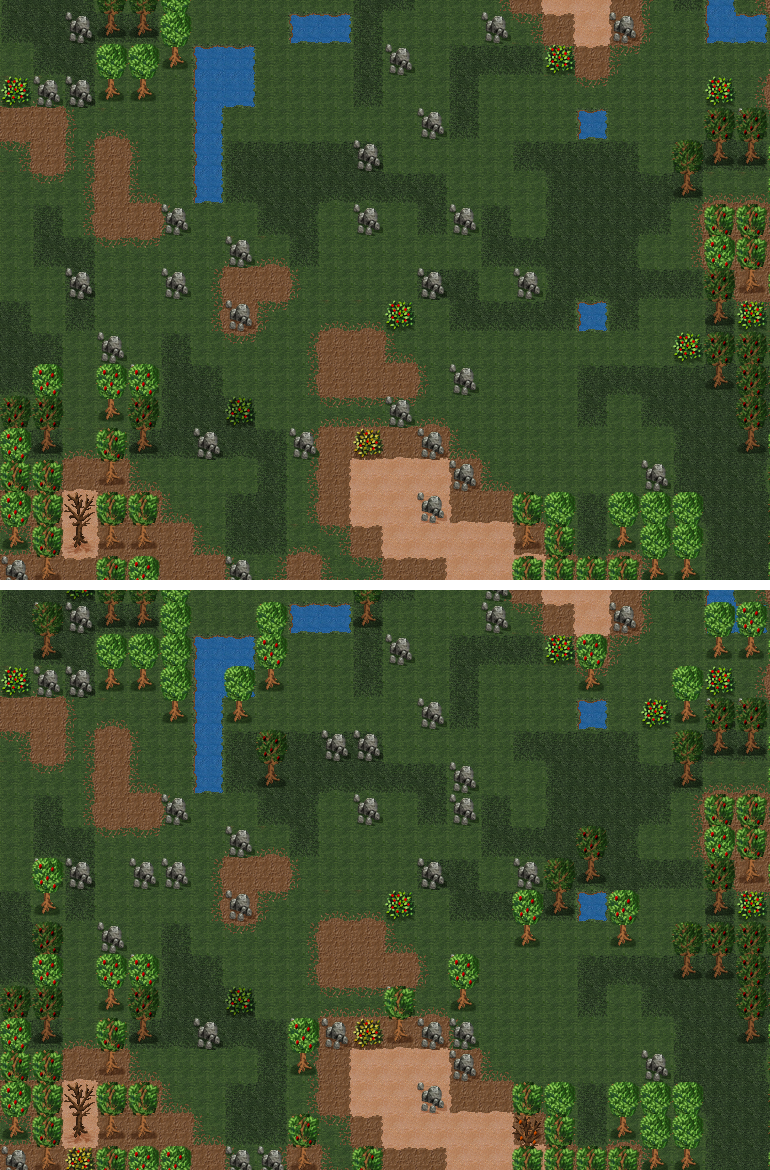
\includegraphics[scale=0.45]{img/SpawnRessource.png}
	  \end{center}
	  \caption{Apparition de tout type de ressource}
	\end{figure}
	\begin{figure}
	  \begin{center}
		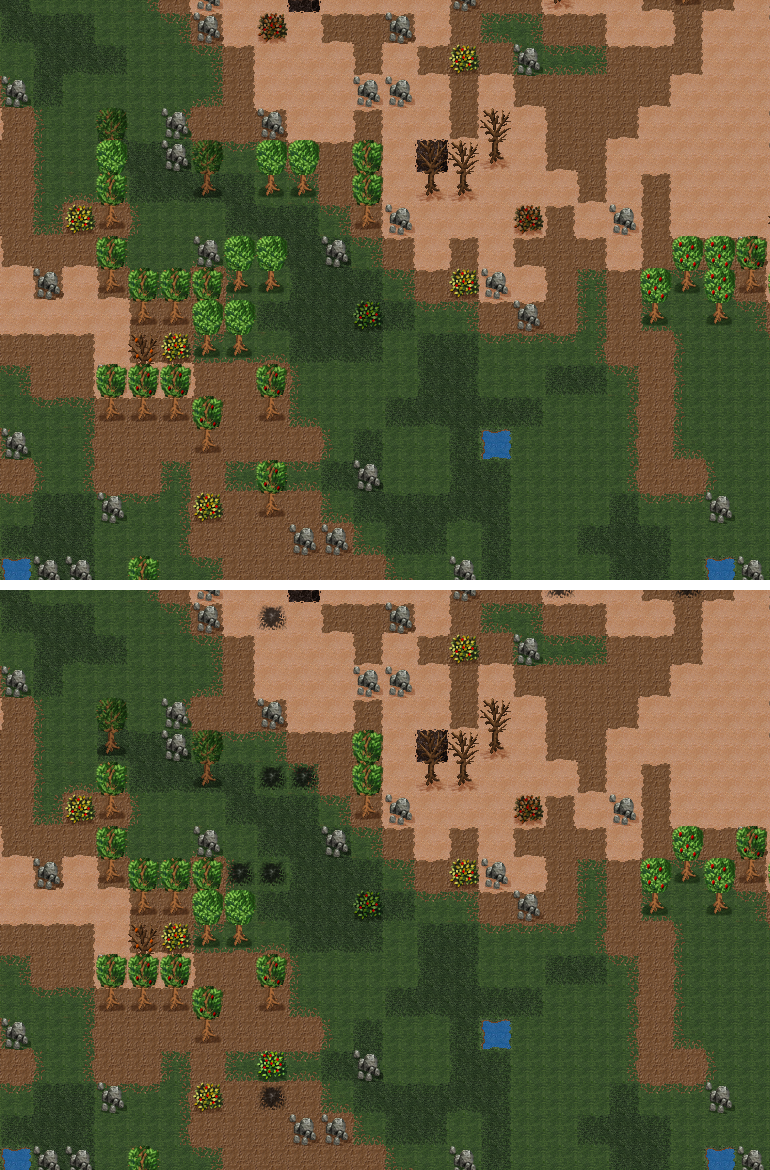
\includegraphics[scale=0.45]{img/BurnRessource.png}
	  \end{center}
	  \caption{Disparition par le feu des ressources contenant du bois}
	\end{figure}
	\begin{figure}
	  \begin{center}
		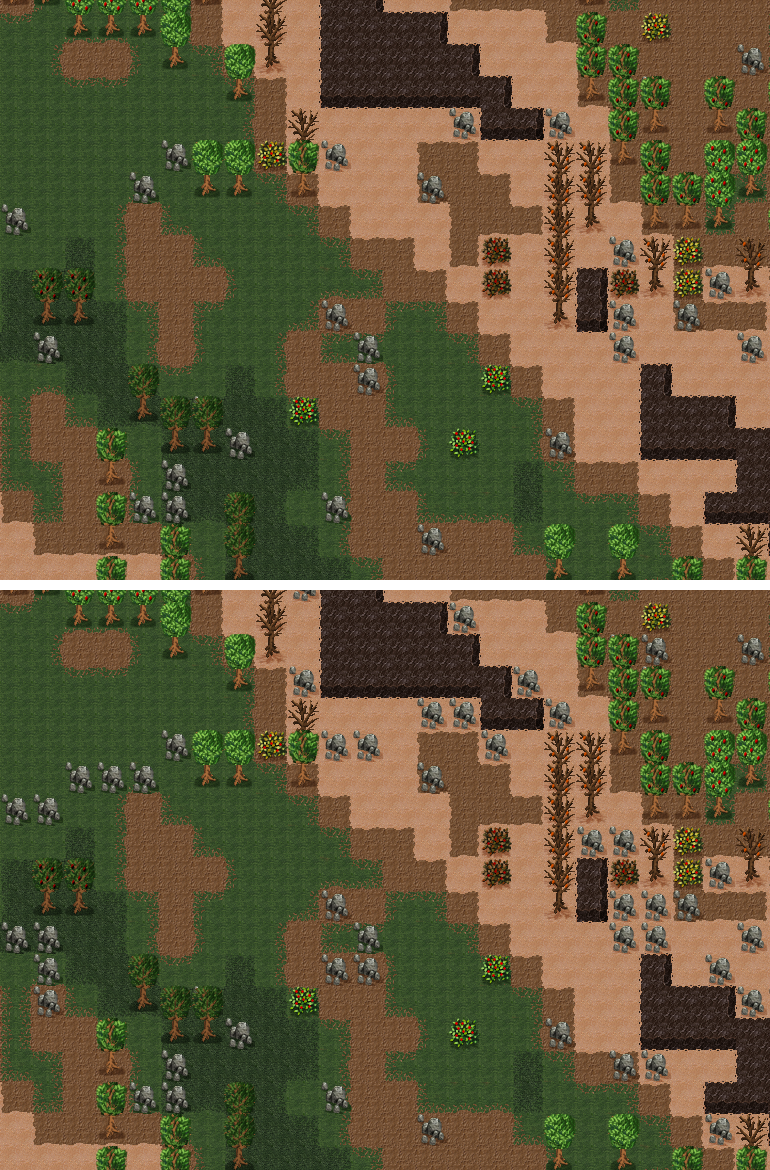
\includegraphics[scale=0.45]{img/SpawnOnlyStone.png}
	  \end{center}
	  \caption{Apparition de rochers uniquement}
	\end{figure}

\end{document}
